\chapter{Úvod}\label{chap:intro}

V tejto úvodnej kapitole by som vás chcel trochu oboznámiť s mojou bakalárkou a poukázať na moju východziu situáciu. Ďalej tiež platformy na ktorých beží a prečo.
\section{Vysvetlenie názvu}
Moja bakalárka sa volá \uv{Optimalizácia obchodovacieho algoritmu na vysoko volatilných komoditných burzách}. Najprv by som tento názov rozobral a podrobne vysvetlil, čo to znamená.
\subsection{Optimalizácia obchodného algoritmu}
Vyvíjame algoritmus, ktorý bude vedieť sám obchodovať. Mojou úlohou bude tento algoritmus testovať a následne optimalizovať aby podával čo najlepšie výsledky.
\subsection{Vysoko volatilných}
Volatilita\cite{Volatilita} je kolísanie. Miera neistoty. A investíciám je vlastná. Platí, že čím vyššie výnosy, tým vyššia volatilita. Z toho vychádza aj pravidlo investičného horizontu, ktorý je pri rizikovejších – teda volatilnejších – aktívach dlhší. Prečo hľadáme  vysoko volatilné burzy ukážem na príklade neskôr.
\subsection{Komoditných burzách}
Náš algoritmus bude pracovať na komoditných burzách, konkrétne na burzách pseudo-mien  hlavne bitcoin. 

\section{Prečo volatilných?}
V tejto časti sa zameriam na okrajové burzy, ktoré sú špecifické svojou vysokou volatilitou
a ukážeme výhody a nevýhody okrajových búrz. Nakoniec zhrnieme, prečo nám vyhovujú práve okrajové burzy.
\subsection{Výhody}
\subsubsection{Vysoká volatilita}
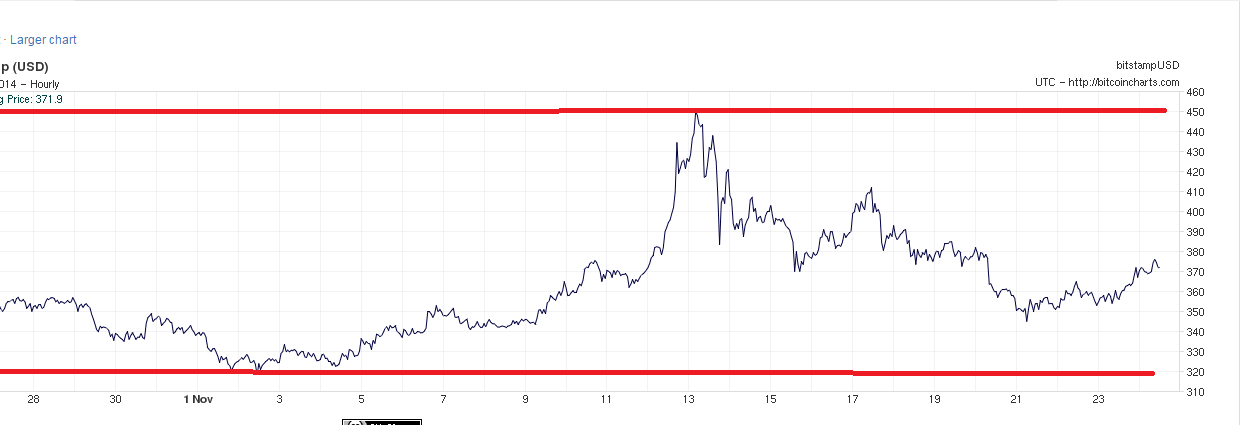
\includegraphics[width=1\textwidth]{obr}
Toto je príklad, keď pozeráme na vysoko volatilnú burzu, ktorou je bitcoin a USD. Možný zisk sa pohybuje až na úrovni 37,5 percenta, keď nerátame poplatky. V prvom obrázku je jeden dielik 10 dolárov. 
\\
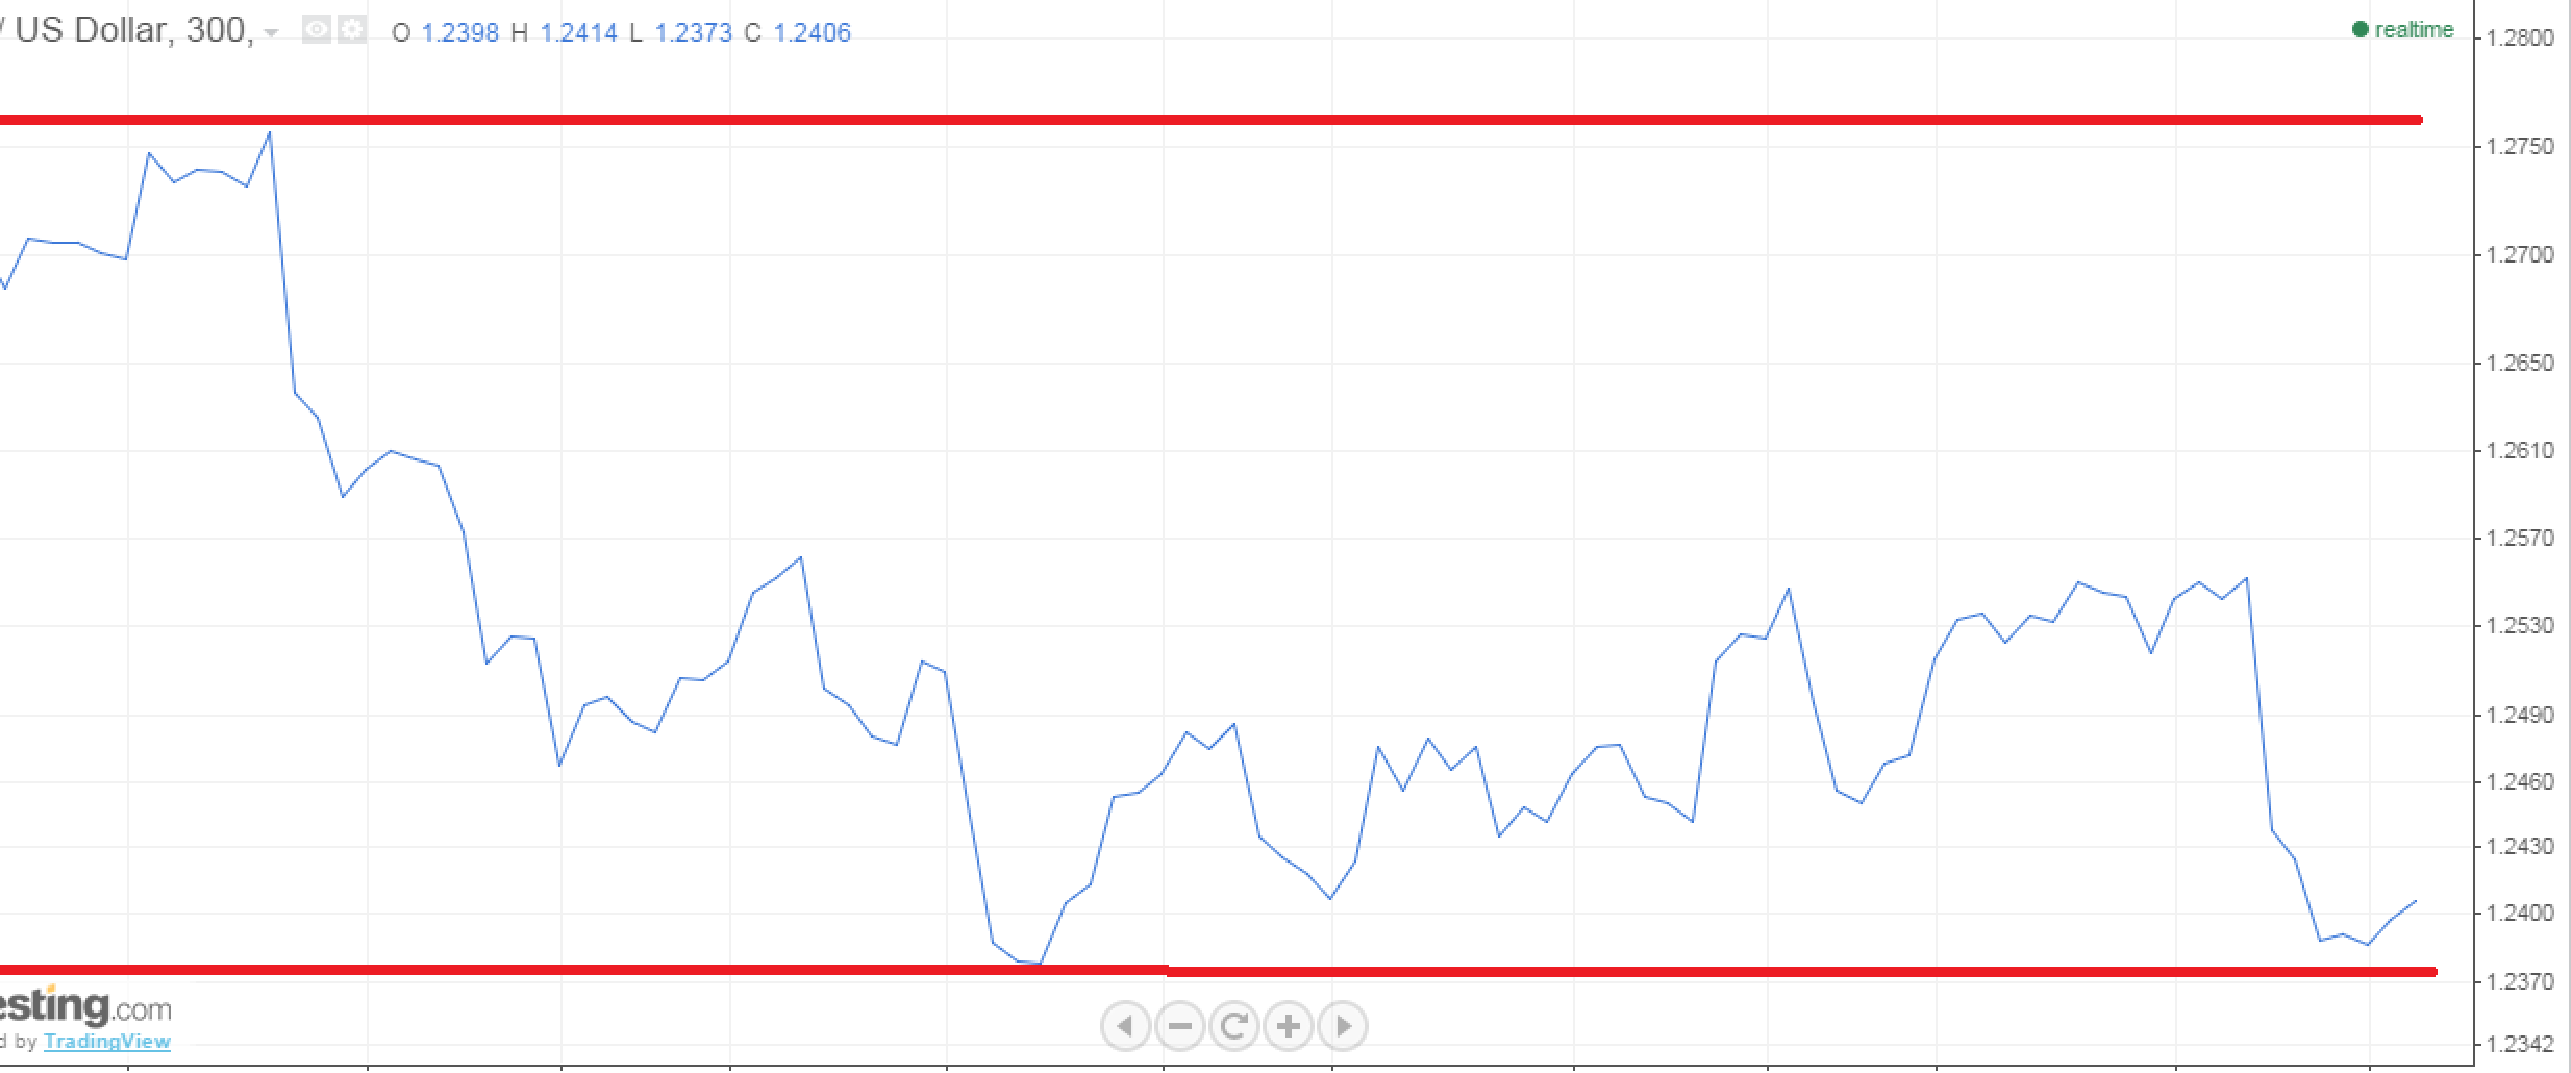
\includegraphics[width=1\textwidth]{obr2}
Na rozdiel od ďalšej málo volatilnej burzy, kde je  možný zisk iba 2,95 percenta a jeden dielik je tisícina danej meny.
\subsubsection{Absencia \uv{Veľkých hráčov}}
Veľký hráči\cite{ZAC} sú hlavne veľké korporácie a bohatí investori. Za to my sme na trhu malí hráči, lebo máme malý kapitál. Ale prečo nie sú na okrajových burzách veľký hráči? Práve preto, že na okrajových burzách sa točí malé množstvo peňazí a na ich investíciách by sa výrazne prejavila likvidita, čo vysvetlím v nevýhodách.
\subsubsection{Nízke poplatky}
Keďže máme malý kapitál, ktorý investujeme, veľmi rýchlo by sme skrachovali, keby poplatok za každú transakciu  bol vysoký. Takže veľkou výhodou na okrajových burzách je, že sa dajú nájsť burzy s minimálnymi vstupnými a inými poplatkami.
\subsection{Nevýhody}
\subsubsection{Veľká likvidita trhu}
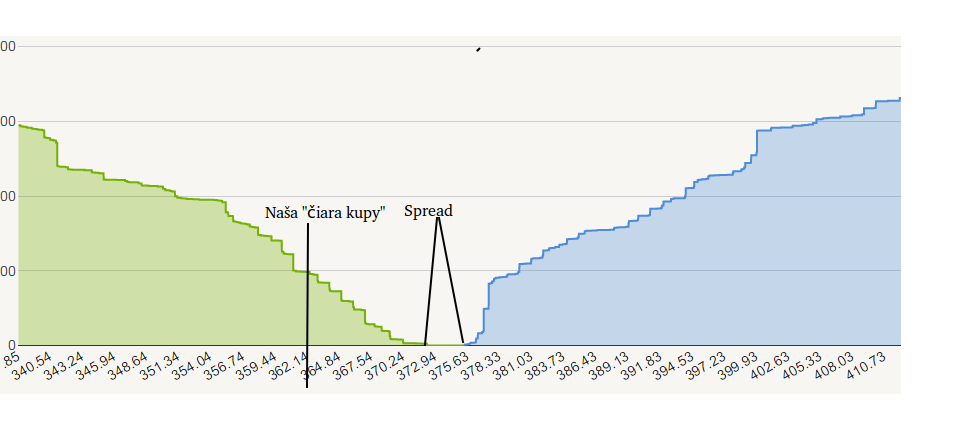
\includegraphics[width=1\textwidth]{stamp}
Najprv vysvetlím pojem \uv{spread}\cite{ZAC}. Spread je rozdiel medzi ponukou a dopytom. Ak je ponuka 1,5 a dopyt 1,6 spread je 0,1. Likvidita trhu vyjadruje zmenu ceny pri obchodoch. Ak je likvidita vysoká, tak veľké investície zmenia cenu meny a naopak ak je nízka veľké obchody s cenou takmer nič neurobia. Súvisí to stým aké veľké množstvo peňazí sa \uv{točí} na burze. Napríklad pozrime sa na obrázok vyššie. Predstavme si že tento trh ma vysokú likviditu. Na obrázku vidíte ponuku, dopyt a spread. 
Ak niekto chce spraviť obchod za 1000 dolárov len malé percento zo sumy kúpi za aktuálny kurz zvyšok drahšie až príde po našu čiaru kúpy. Dokým trh nezareaguje vznikne obrovský spread a tiež to zamáva s kurzom. Veľkým hráčom sa neoplatí obchodovať na okrajových burzách, pretože by to pri veľkých investíciach nebolo výhodné.
\subsubsection{Väčšie riziko}
Na okrajových burzách je väčšie riziko že svoje investícii stratíš bez tvojho pričinenia. Či sa burza zrazu vyparí za záhadných okolnosti alebo ju niekto \uv{vybrakuje} a už nič nezostane pre teba. Stalo sa v nedávnej minulosti že významné okrajové burzy, zo dňa na deň zmizli a ľudia prišli o svoje investície.  
\subsection{Zhrnutie}
Z toho čo som vyššie napísal je zjavné,  že pre naše zámery je okrajová burza ideálna. Keďže naše investície do burzy nie sú veľké, veľkou výhodou sú pre nás nízke poplatky a malou nevýhodou vysoká likvidita. Z rizikom že prídeme zo dňa na deň o všetko sa musíme zmieriť. Tiež absencia veľkých hráčov nám vyhovuje, lebo tí by mohli stabilizovať burzu a tým pádom by sme prišli o vysokú volatilitu, ktorá je pre nás výhodou. Ktoré burzy(platformy) vyhovujú našim požiadavkám uvediem ďalej.
\section{Vyhovujúce platformy}

